\documentclass[a4paper,12pt]{article}
\usepackage{fancyhdr}
\usepackage{lastpage}
\usepackage{geometry}
\usepackage{listings}
\usepackage{datetime}
\usepackage{xeCJK}
\usepackage{hyperref}
\usepackage{amsmath}
\usepackage{graphicx}
\usepackage{float} % 加入 float 宏包以使用 [H]
\usepackage{longtable}

\geometry{left=2.5cm, right=2.5cm, top=2.5cm, bottom=2.5cm}
\pagestyle{fancy}
\setCJKmainfont{Noto Sans TC}
% 英文字體 consolas
\setmonofont{Consolas}
% 設定內文文字大小
\renewcommand{\normalsize}{\fontsize{12pt}{\baselineskip}\selectfont}

% 設定頁首
\fancyhf{}
\fancyhead[L]{Volume Rendering and Gradient Visualization(HW2)}
\fancyhead[R]{\today}
\fancyfoot[C]{\thepage/\pageref{LastPage}}

\title{Volume Rendering and Gradient Visualization(HW2)}
\author{01057033洪銘均}
\date{\today}

\begin{document}
\maketitle
\tableofcontents
\newpage

\section{程式概述}
該程式利用2D的視覺化方式將vector field變成Stream Line以及呈現,Stream Line計算使用了RK4來繪製點的位置,並且利用IMGUI可以設定Steam Line參數,另外有使用Line Integral Convolution來做底圖,可以透過IMGUI切換是否顯示


\section{運行結果}

\begin{figure}[h]
    \centering
    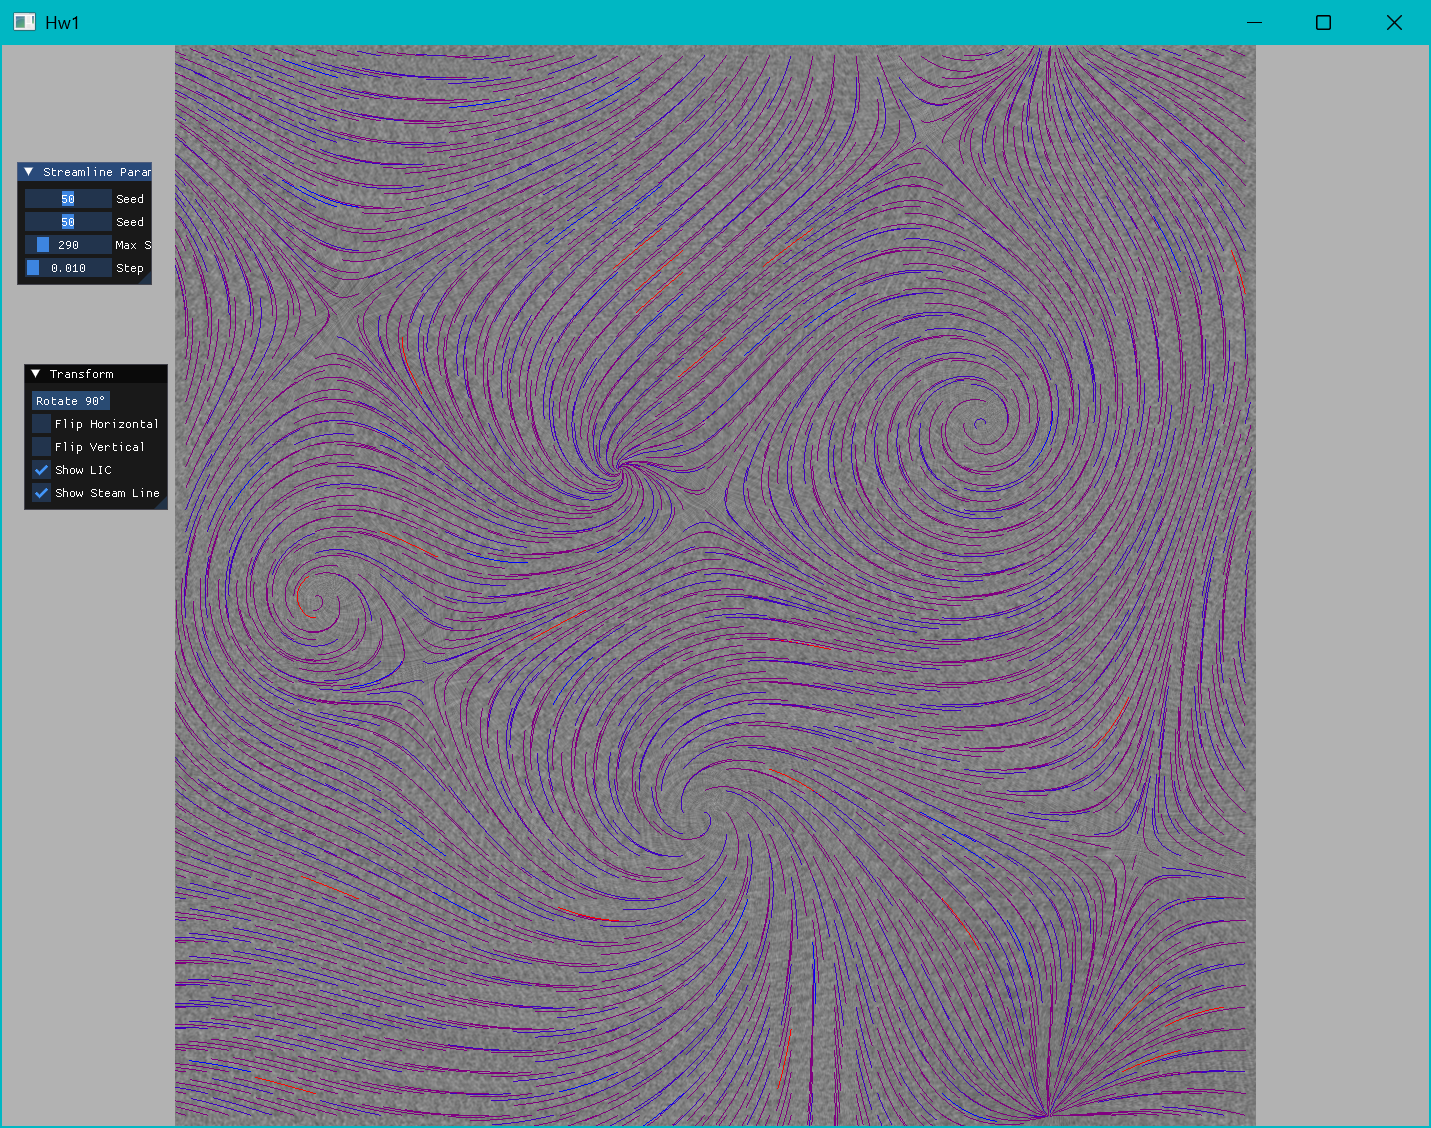
\includegraphics[width=0.8\textwidth]{img/img0.png}
\end{figure}
圖為使用Stream Line作為上層圖層、LIC image為下層圖層,可以看到上下層顯示出來線條大致相同,並且紅色為梯度較高的區域,藍色為較低的區域

\begin{figure}[h]
    \centering
    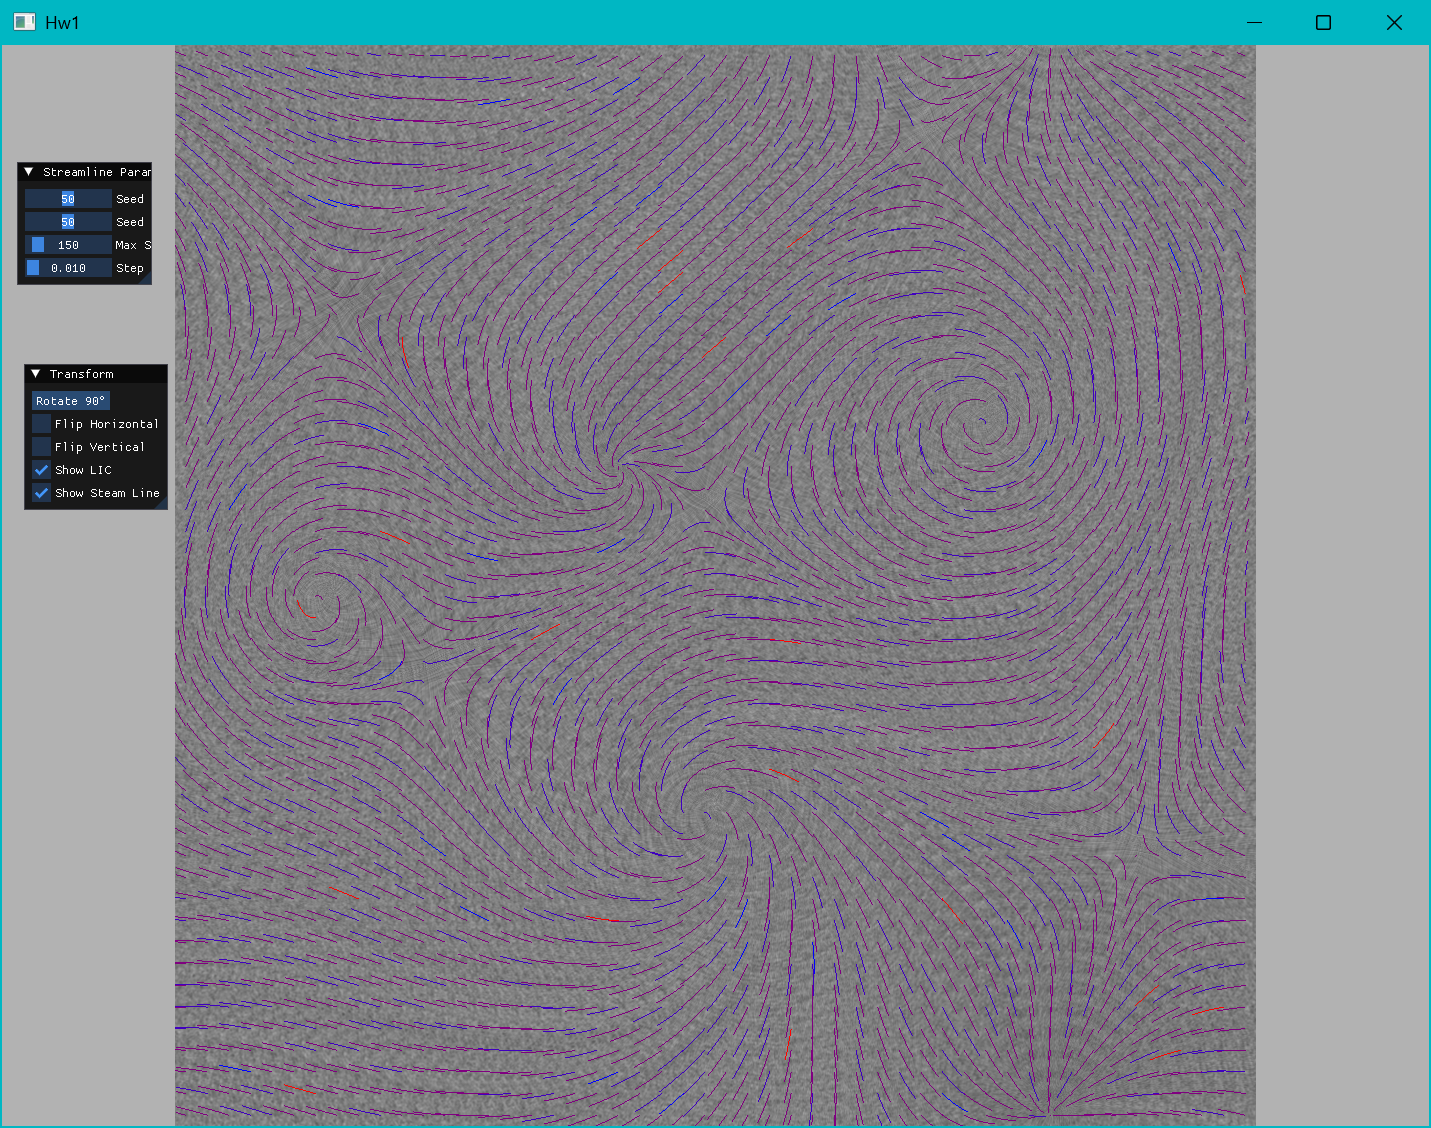
\includegraphics[width=0.8\textwidth]{img/img1.png}
\end{figure}
圖中為設定不同的Max Steps數值後的結果,可以看到流線長度明顯不同

\begin{figure}[h]
    \centering
    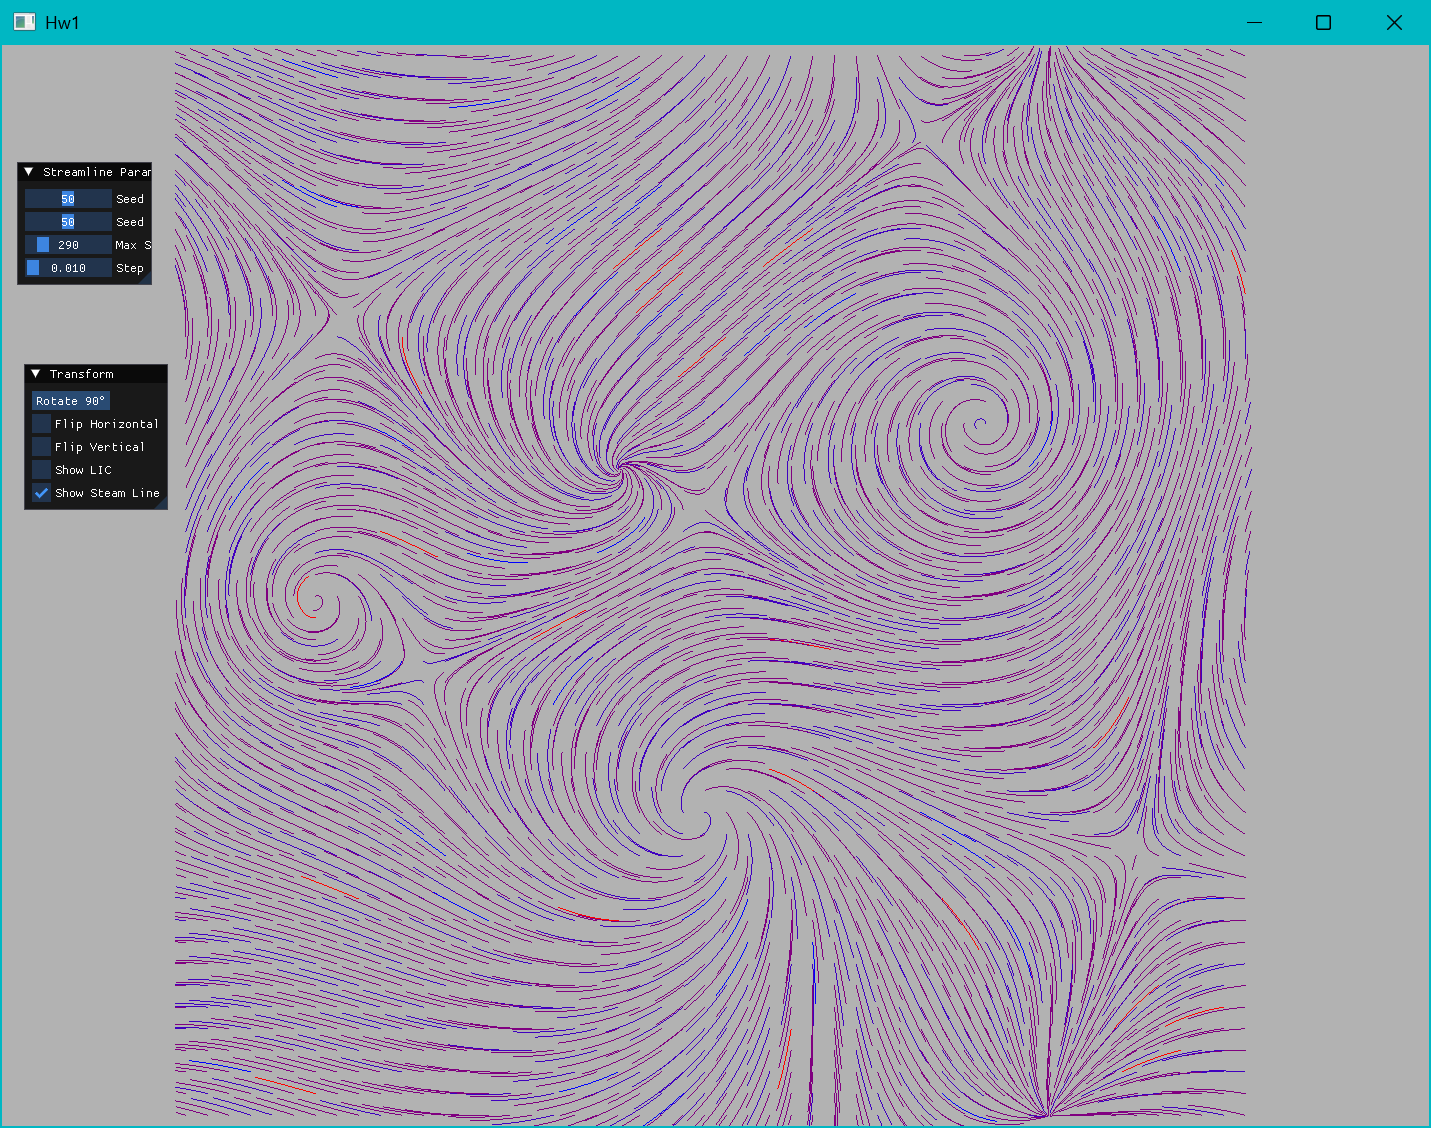
\includegraphics[width=0.8\textwidth]{img/img2.png}
\end{figure}
圖中為Stream Line圖層

\begin{figure}[h]
    \centering
    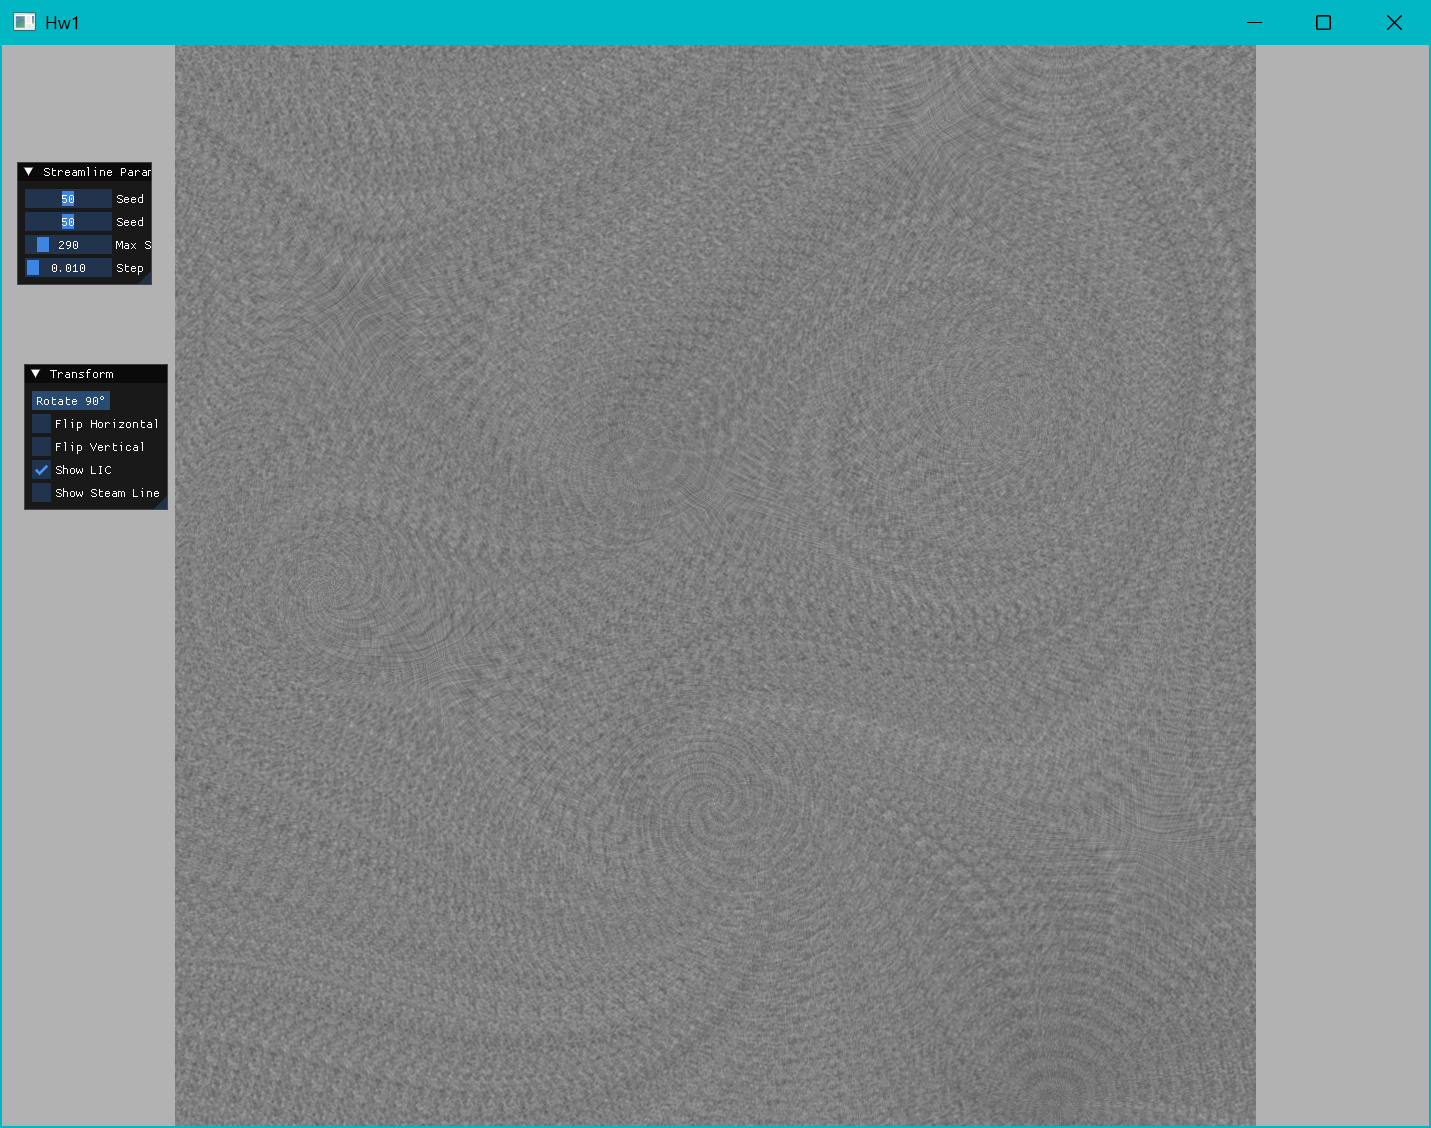
\includegraphics[width=0.8\textwidth]{img/img3.png}
\end{figure}
圖中為Line Integral Convolution圖層



\section{心得}
    這次作業成功了解到如何將Vector Field做視覺化,平常就有在看天氣,有看到風場和洋流場的流線視覺化,但也都不知道是如何去實現的,這次作業也算是完全理解氣象視覺化的方式,並且也將之前數值分析就講過的RK Method給實做出來。
\end{document}

% xelatex  --max-print-line=10000 -synctex=1 -interaction=nonstopmode -file-line-error -recorder .\codebook.tex 
